\section{Evolution of spinless BEC under speckle pulsing}\label{speckle_pulsing}
In Ch.~(\ref{speckle_chapter}), we derived a Gaussian beam model of the speckle beam and calculated the field-field correlation function, the PSD, and the intensity distribution. In the experiments, the engineered speckle beam is focused at the atoms and it is hard to directly measure the average intensity of the speckle beam at the atoms. Direct measurements of the PSD and $k_c$ is even harder. In some experiments carried out previously that involved a speckle beam \cite{kondov2011three, billy2008direct}, the researchers set up an identical beam at the test bench and measure the average intensity and the PSD of the test speckle beam. The power and the PSD of the speckle beam in the experiments are assumed to be the same as those of the test beam, but no direct measurements were done to the best of our knowledge. Inspired by \cite{huckans2009quantum}, we designed and carried out an experiment that allowed us to measure the average intensity and the PSD of the speckle beam by using the evolution of spinless BECs under the speckle potentials.

\begin{figure*}
    \centering
    \includegraphics{Chapter6_secs/speckle_pulsing_images.pdf}
    \caption{Absorption images of atoms after the evolution under speckle potentials and TOF. The BECs are released from the dipole trap, the pulses of the speckle potentials are turned on immediately for a various amount of time, followed by TOF. The absorption images are stacked up horizontally according to the speckle pulse duration.}
    \label{fig:speckle_pulsing_imgs}
\end{figure*}

In \cite{huckans2009quantum}, the diffraction of a Bose-Einstein condensate from a one-dimensional optical lattice is studied. In very short time,
\begin{equation}
    T_{pulse} \ll t_{RN} = \frac{\hbar}{\sqrt{U_0E_L}} = \frac{T_{ho}}{\pi},
\end{equation}
the atoms are mainly scattered to the $\ket{\pm k_L}$ momentum states. Since in the Raman-Nath approximation, the atoms move by a very small distance, the kinetic energy term in the Hamiltonian is neglected. The atomic momentum changes from $\ket{k=0}$ to $\ket{\pm k_L}$, which corresponds to the nonzero components in the PSD of the lattice potential. This inspires us to measure the PSD of the speckle potential and the cutoff $k_c$ by using the short-term speckle beam pulses.

As the pulse duration increases beyond $t_{RN}$, the apparent edge of the momentum distribution is bounded by a maximum momentum $k_{max}$. The observed value of $k_{max}$ can be used to determine the lattice depth $U_0$,
\begin{equation}
    U_0 = \frac{\hbar^2k_{max}^2}{2M}
\end{equation}
Once the edge of the distribution reaches $k_{max}$, the distribution partially collapses to $\ket{k=0}$ at $T_{ho}/2$. The process approximately repeats itself every $T_{ho}/2$. The collapse and revival phenomena can be qualitatively explained in a classical picture. The atoms released from different positions in a harmonic trap become stationary every half of the period. The collapse and revival are not complete in \cite{huckans2009quantum}, at $T_{ho}/2$ there are always some higher momentum orders remain. The reason is that the lattice potential is not perfectly harmonic. 

In contrast to the lattice pulsing, in the speckle beam pulsing, the speckle potential contains a continuous spectrum of spatial frequency. It is completely anharmonic and no collapse and revival should be expected. For long speckle pulsing time, the momentum states should reach a stationary distribution. By Virial theorem, the kinetic energy of the atoms under this stationary distribution should be half of the average speckle potential. This inspired us to measure the average speckle potential by using the width of the momentum distribution for a long speckle pulsing time.

% \begin{figure*}
%     \centering
%     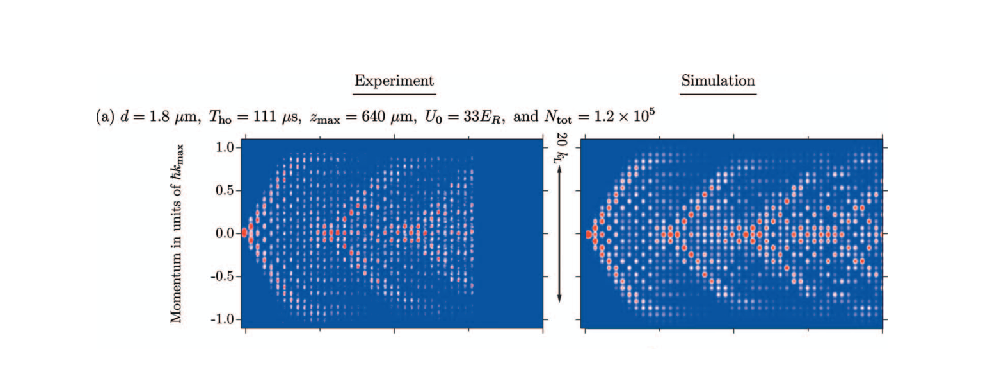
\includegraphics{Chapter6_secs/lattice_pulsing.pdf}
%     \caption{Fig.~1(a) of \cite{huckans2009quantum}. Concatenated absorption images of diffraction patterns, showing the evolving momentum distribution, compared with numerical GPE simulation results.}
%     \label{fig:lattice_pulsing}
% \end{figure*}

\subsection{Short term speckle pulsing}\label{short_pulse_sec}

To measure the PSD and the cutoff $k_c$ of the speckle potentials with short term speckle pulsing, we derive the evolution of the momentum states under two approximations. The first is the Raman-Nath approximation, atoms do not move far during the pulse.  The second is that the evolution time is short compared to $\hbar/V(x)$, so atoms do not acquire a phase comparable to $2\pi$.
Consider Hamiltonian
\begin{equation}
    \hat{H} = \frac{\hbar^2k^2}{2m} + V(x).
\end{equation}
The time evolution operator is
\begin{equation}
    \hat{U}(t) = \exp{-i\frac{\Delta t}{\hbar}\left[\frac{\hbar^2k^2}{2m}+V(x)\right]},
\end{equation}
Define $E_c$ as the energy associated with $k_c$, $\tau = \frac{\Delta t}{\hbar}E_c$, $\hat{k} = \frac{k}{k_c}$ and $S(x) = \frac{V(x)}{E_c}$
\begin{equation}
    \hat{U}(t) = \exp{-i\tau\left[\hat{k}^2+S(x)\right]}.
\end{equation}
Expand the operator to second order, 
\begin{equation}
    \hat{U}(t) = \exp{-i\tau\hat{k}^2/2}\exp{-i\tau S(x)}\exp{-i\tau\hat{k}^2/2}.
\end{equation}
We assume the initial state is $\ket{k=0}$, so the third term does not contribute. And we measure the distribution in $k$ space, so we can ignore the first term. The second term governs the short time evolution. To the lowest order, 
\begin{equation}
    \hat{U}(t)\ket{k=0} = \ket{k=0} - i\tau S(x) \ket{k=0}
\end{equation}
Expand $S(x)$ in $k$ space,
\begin{equation}
    S(x) = \sum_{k,k'}\Tilde{S}(k-k')\dyad{k}{k'}
\end{equation}
So
\begin{equation}
    \hat{U}(t)\ket{k=0} = \ket{k=0} - i\tau \sum_{\delta k}\Tilde{S}(\delta k)\ket{\delta k}
\end{equation}
The probability distribution of momentum states at time $\tau$ is
\begin{equation}\label{short_dist}
    P(k,\tau) = \tau^2 |\Tilde{S}(k)|^2 + \delta_{k,0}.
\end{equation}
It is proportional to the PSD of the speckle potential $|\Tilde{S}(k)|^2$ ignoring the central peak at $k=0$.

In the experiments, we put an iris right before the diffuser $D$ in \ref{fig:design}. By opening and closing the iris, we can control the size of the beam which determines $k_c$ of the speckle potential PSD in the focal plane. As the model we derived in Ch.~(\ref{speckle_chapter}) shows, the speckle beam size at the focal plane does not change with the beam size at the diffuser. The beam size at the focal plane is determined by the field-field correlation length at the diffuser. So the average speckle potential depth is proportional to the power of the beam which we can control when we change the size of the iris. 

We did the experiments for two iris sizes, $6.5\ {\rm mm}$ and $15\ {\rm mm}$, which correspond to $k_c=0.65k_r$ and $k_c=1.30k_r$, respectively. Here $k_r$ is defined with the largest recoil $k$ vector of atoms scattered by a $532\ {\rm nm}$ light beam focused by a one inch $f=30\ {\rm mm}$ lens. 
\begin{equation}
    k_r = \frac{2\pi}{532 {\rm nm}}\sin{\frac{\theta_{\rm R}}{2}}
\end{equation}
$\theta_{\rm R} \approx 45^\circ $ is shown in Fig.~(\ref{fig:raman_design}).
The average speckle potential match in both cases by controlling the power of the beam after the iris. 

We prepare BECs in a cross dipole trap, at $t=0$, we turn off the dipole trap and release the atoms for time-of-flight (TOF). Immediately after the dipole trap is turned off, we turn on the speckle beam and pulse for a short period of time, ranging from $20\ {\rm \mu s}$ to $250\ {\rm \mu s}$. After $18\ {\rm ms}$ TOF, we take absorption images of the atoms.

To compare with the experimental data, we simulate the process numerically. In the numerical simulation, we prepare the ground state of BECs in a dipole trap. At $t=0$, turn off the dipole trap and release the atoms. Immediately after, the speckle potential is turned on for a duration of $50\ {\rm \mu s}$ or $100\ {\rm \mu s}$, followed by free evolution for up to $20\ {\rm ms}$. We keep track of the momentum distribution of the atoms during the evolution. 

\begin{figure*}
    \centering
    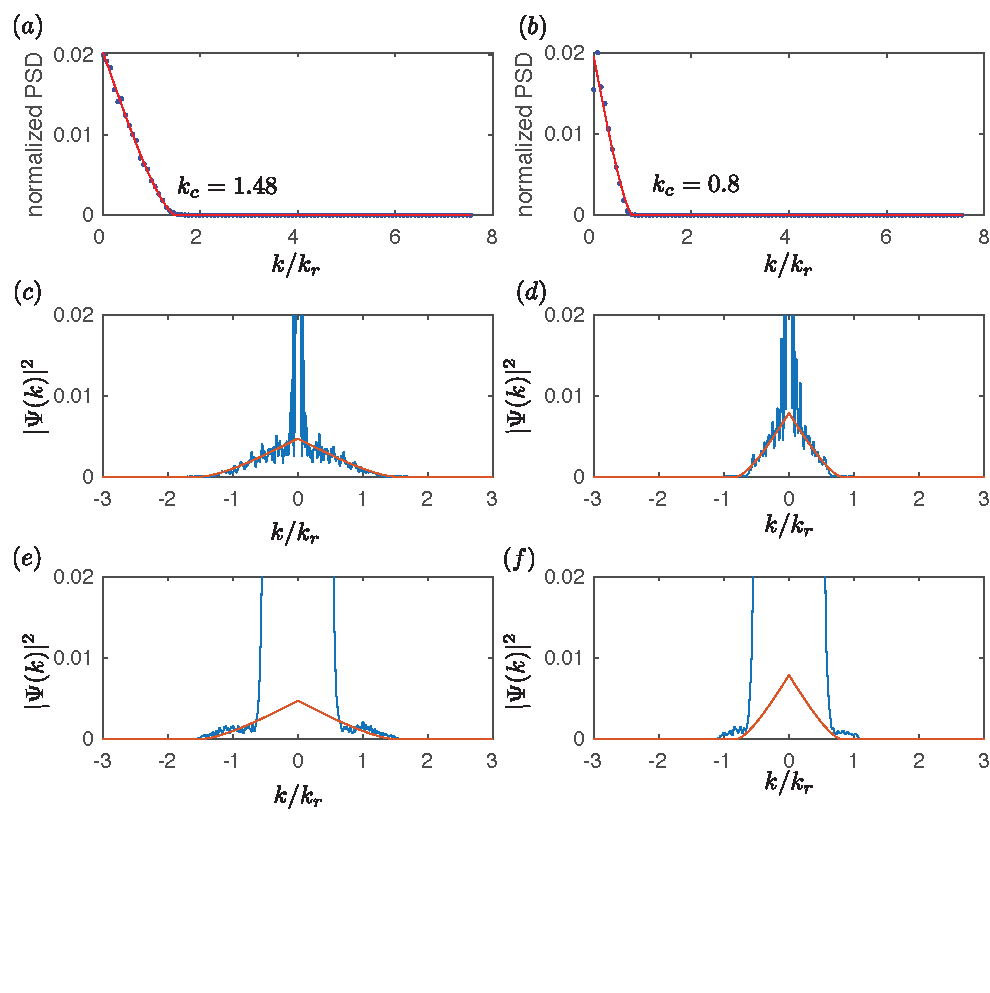
\includegraphics{Chapter6_secs/speckle_pulsing_simu.pdf}
    \caption{Simulation of short-term speckle pulsing. The left panel is for speckle potential with $k_c = 1.48k_r$, and the right panel for $k_c = 0.8k_r$. (a) and (b) verify the $k_c$ of both speckle potentials by plotting their PSD. (c) and (d) are the momentum distribution of atoms after released from the dipole trap and evolve under speckle pulses for $50\ {\rm \mu s}$. The red curves are proportional to the corresponding PSD of the speckle potential. The momentum distribution is an average of 20 speckle realizations. (e) and (f) are the momentum distribution of atoms after released from the dipole trap and evolve under speckle pulses for $50\ {\rm \mu s}$ followed by a $20\ {\rm ms}$ free expansion. The results are averaged over 20 speckle realizations. }
    \label{fig:speckle_pulsing_simu}
\end{figure*}

As Fig.~(\ref{fig:speckle_pulsing_simu}) shows, the simulation is done under two kinds of speckle potentials with different $k_c$ to compare with the experimental data. The left panel of Fig.~(\ref{fig:speckle_pulsing_simu}) is for the speckle potential with $k_c = 1.48k_r$ and the right panel for the speckle potential with $k_c = 0.80k_r$. Fig.~\ref{fig:speckle_pulsing_simu}(c) and Fig.~\ref{fig:speckle_pulsing_simu}(d) show the momentum distribution of atoms immediately after a $50\ {\rm \mu s}$ speckle pulsing, the results are averaged over 20 speckle realizations. The red curves are proportional to the PSD of the two kinds of speckle potentials, respectively. From Fig.~\ref{fig:speckle_pulsing_simu}(c) and Fig.~\ref{fig:speckle_pulsing_simu}(d) we can see the tail of the momentum distribution of atoms after short-term speckle pulsing matches with the PSD of the speckle potentials. The results agree with the analytical calculation of the momentum distribution in Eq.~(\ref{short_dist}), which predicts the momentum distribution to be a central $\delta$ function plus a tail that is proportional to the PSD of the speckle potentials. 

Fig.~\ref{fig:speckle_pulsing_simu}(e) and Fig.~\ref{fig:speckle_pulsing_simu}(f) show the momentum distribution of atoms after a $50\ {\rm \mu s}$ speckle pulse and a $20\ {\rm ms}$ time-of-flight (TOF). During the TOF, the mean-field expansion of the atoms broadens the momentum distribution. Both the central peak and the tail of the momentum distribution become broader after the TOF. In Fig.~\ref{fig:speckle_pulsing_simu}(f), for the speckle potential of smaller $k_c$, the tail of the momentum distribution is broadened more significantly. The broadened momentum distribution after TOF makes it harder to distinguish the speckle potentials with the tail of the momentum distribution.

\begin{figure*}
    \centering
    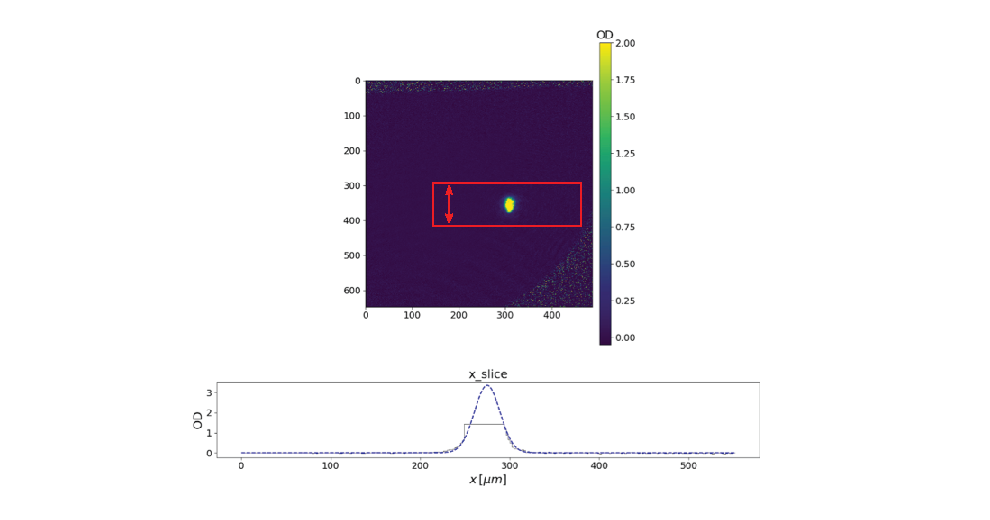
\includegraphics{Chapter6_secs/colOD.pdf}
    \caption{A sample of absorption images of atoms and analysis. The red square is a selected region of interest and the red arrow indicates the direction we take average. The masked and averaged spatial distribution of atoms (black curve) and a fitted Gaussian curve (blue dashed) are plotted below.}
    \label{fig:colOD}
\end{figure*}

\begin{figure*}
    \centering
    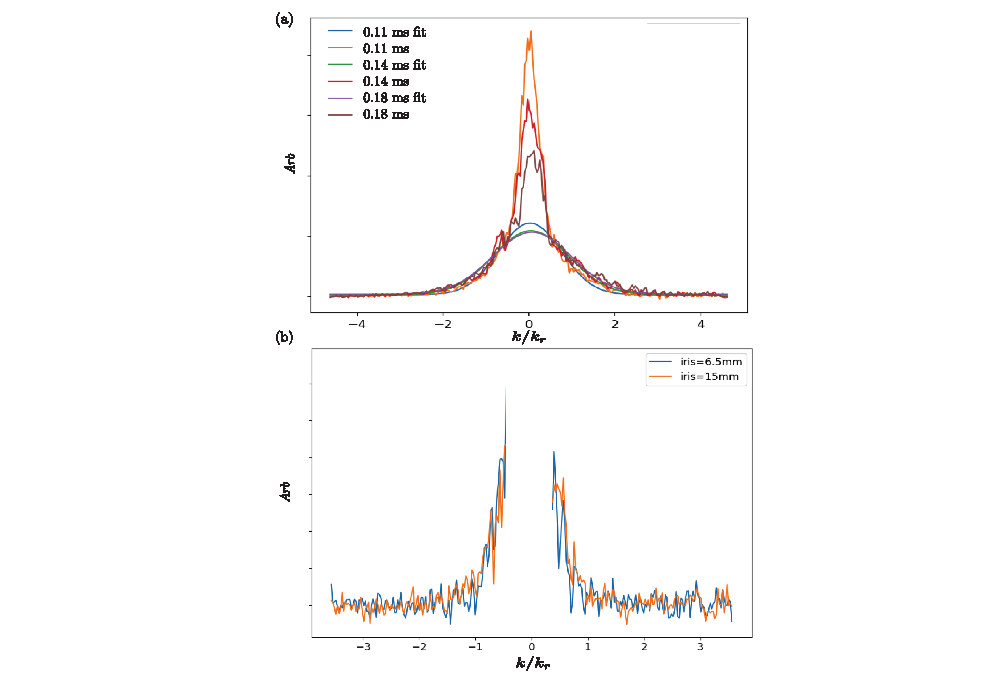
\includegraphics{Chapter6_secs/short_pulse.pdf}
    \caption{Momentum distribution after short-term speckle pulses and $18\ {\rm mm}$ TOF. (a). A few samples of momentum distribution of atoms without mask, along with fitted Gaussian curves to the masked momentum distribution. (b). The tails of the momentum distribution after short-term pulses of speckle potential with different PSD. The PSD of the speckle potentials are controlled by the iris sizes and the results are averaged for speckle pulsing time ranging from $80\ {\rm \mu s}$ to $150\ {\rm \mu s}$.}
    \label{fig:short_pulse}
\end{figure*}


Fig.~\ref{fig:colOD} and Fig.~\ref{fig:short_pulse} show the analysis results of the absorption images after TOF for two kinds of speckle potentials generated with different iris sizes. During TOF, the momentum distribution of atoms is mapped to their spatial distribution. From the absorption images, we can compute the momentum distribution from the spatial profile of the atoms. In the analysis, from the absorption images of atoms after TOF shown in Fig.~\ref{fig:colOD}, we select a region of interest around the center of the atoms indicated by the red square. And compute the average spatial distribution of atoms along the horizontal direction (red arrow). The central peak of this average spatial distribution is masked to show the detail of the tails. Fig.~\ref{fig:colOD} shows an example of the masked averaged spatial distribution along $x$ direction (black curve) and a Gaussian fit (blue dashed curve). The resultant tails of the spatial distribution are averaged over short-term speckle pulsing duration ranging from $80\ {\rm \mu s}$ to $150\ {\rm \mu s}$. The tails of the spatial distribution are then converted to that of the momentum distribution in a unit of $k_r$. 


Fig.~\ref{fig:short_pulse}(a) shows a few samples of the averaged momentum distribution along $x$ direction without a mask for short-term speckle pulsing, along with fitted Gaussian curves to the masked momentum distribution. From Fig.~\ref{fig:short_pulse}(a) we can see it is necessary to mask the central peak of the momentum distribution in order to analyze the width of the tails. Fig.~\ref{fig:short_pulse}(b) is the momentum distribution of atoms after short-term pulses of speckle potentials with different PSD, averaged over pulsing duration ranging from $80\ {\rm \mu s}$ to $150\ {\rm \mu s}$. From Fig.~\ref{fig:short_pulse}(b), it is hard to tell the difference between the two curves for two reasons. First, in the absorption images, the signal-noise-ratio at the tails of the density profile is low. Just by taking the average, it is hard to reduce the noise and see the clear tails as in the numerical simulation in Fig.~\ref{fig:speckle_pulsing_simu}. Second, as the simulation results show in Fig.~\ref{fig:speckle_pulsing_simu}(e) and Fig.~\ref{fig:speckle_pulsing_simu}(f), during TOF, the mean-field expansion broadens the momentum distribution more significantly for speckle pulsing with smaller $k_c$. So the width of the tails of the momentum distribution for the pulsing of two kinds of speckle potentials is closer to each other after TOF than before. For the two reasons, we conclude we can not quantitatively measure the $k_c$ of the speckle potential by using the absorption images after short-term speckle pulsing and TOF.



\subsection{Long term speckle pulsing}\label{long_pulse}

In the experiments, it is important to know the average speckle potential at the atoms. But unfortunately, it is hard to measure the power of the speckle beam directly at the atoms and infer the average speckle potential. Because in the experiments, we can not put a power meter anywhere we want to measure the power of the beam. And besides, it is the intensity that matters, and we don't have perfect knowledge of the beam size at the atoms. After the closest point to the vacuum glass cell where we can use a power meter to measure the power, the beam goes through lenses, reflected by mirrors, glass cell or even dichroic mirrors. The power of the beam decreases at each of the optical element. To the best of our knowledge, for the previous experiments using speckle beams, the average speckle potential was not measured directly. It could be inferred by calculating the power given the power loss at each optical element. Or the power could be measured for an identical speckle beam set up on the test bench and it is assumed the power at the atoms is the same as the power of the test speckle beam in the focal plane. 

Inspired by \cite{huckans2009quantum}, we obtained the mean potential depth by making the atoms evolve under the speckle beam pulses. Compared with \cite{huckans2009quantum}, for $t \gg t_{RN}$, we do not expect to see the collapse and revive phenomenon due to the anharmonicity of the speckle potential. Instead, at long speckle pulsing time, the momentum distribution should reach equilibrium and by virial theorem, the average stationary kinetic energy is half of the average total energy which is the initial average speckle potential. 

To confirm our understanding, we did numerical simulations of the long-term speckle pulsing. Fig.~\ref{fig:speckle_pulsing} shows the simulation and experimental results of the speckle pulsing for the pulsing duration up to $2\ {\rm ms}$. In the simulation, we release the BECs from the dipole trap and immediately turn on the speckle potential. The atoms evolve under the speckle potential and we keep track of the width of the momentum distribution. We did the simulation for different average speckle potential depth ranging from $0\ {\rm Hz}$ to $1600\ {\rm Hz}$, with a $200\ {\rm Hz}$ spacing. The results are shown as the nine curves, each one is averaged over 20 speckle realizations. When the average speckle potential is zero, the width of the momentum distribution increases driven by the mean-field expansion. From the simulation results shown in Fig.~\ref{fig:speckle_pulsing}(a), the width of the momentum distribution increases rapidly after the speckle potential is turned on and becomes stationary after around $0.25\ {\mu s}$. The stationary width increases with the average speckle potential depth. Fig.~\ref{fig:speckle_pulsing}(b) shows the experimental results. In the experiment, we release the atoms from the dipole trap, pulse the speckle potential for up to $2\ {\rm mm}$ followed by TOF. The total time for the speckle pulsing and the TOF is $18\ {\rm ms}$, a constant for different pulsing duration. We take the absorption images after TOF and fit a Gaussian function to the density profile of the atoms. Fig.~\ref{fig:speckle_pulsing}(b) shows the width of the fitted Gaussian function vs the duration of the speckle pulses. The Gaussian width increases with the pulsing duration in short term and becomes stationary after around $0.25\ {\rm ms}$, which is consistent with the simulation results. 

\begin{figure*}
    \centering
    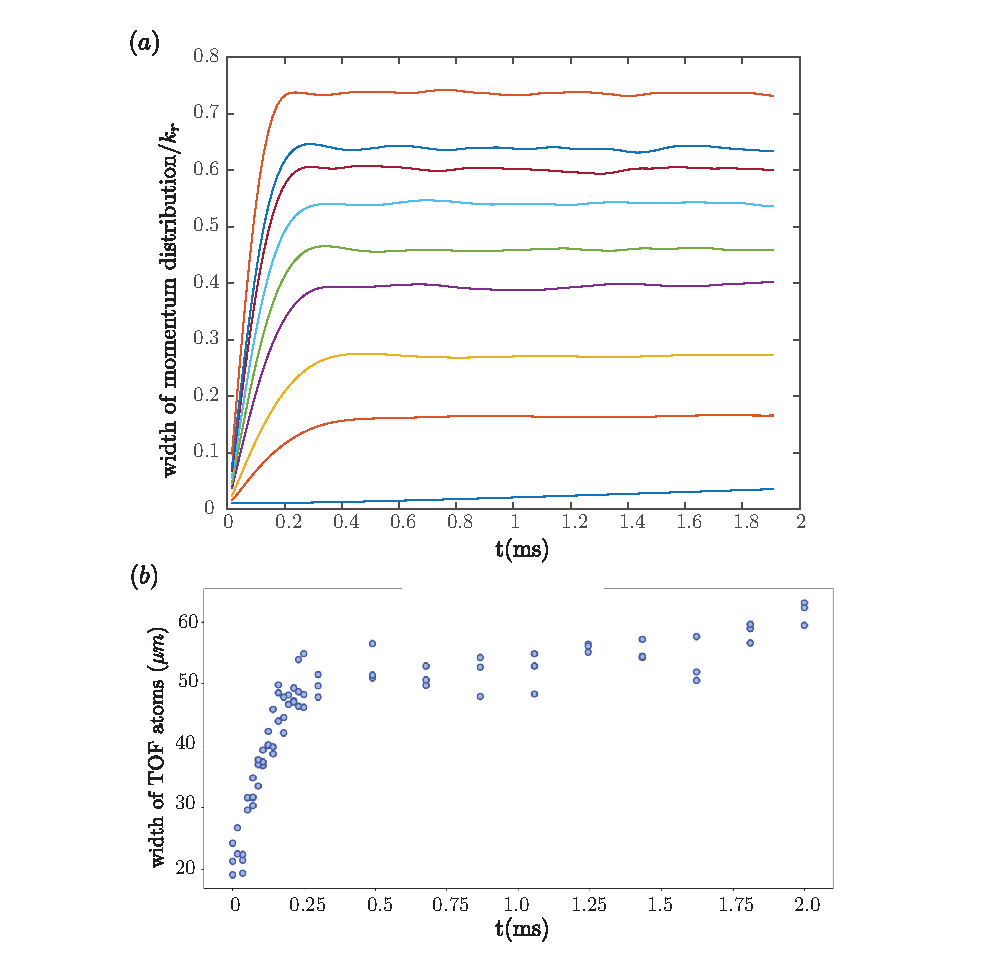
\includegraphics{Chapter6_secs/speckle_pulsing_width.pdf}
    \caption{The simulation and the experiments of the speckle beam pulsing. (a). The width of the momentum distribution of atoms evolving under the speckle potentials of different potential depth ranging from $0$ to $1600\ {\rm Hz}$.  (b). The Gaussian width of atoms in the absorption images after TOF for different speckle pulsing duration.}
    \label{fig:speckle_pulsing}
\end{figure*}

To infer the average speckle potential from the width of the momentum distribution after long-term speckle pulsing, we compute the average kinetic energy using the fitted Gaussian width of the density profile of atoms after TOF.
\begin{equation}
    \langle \hat{K} \rangle = \frac{1}{2} m \left(\frac{\sigma}{\tau}\right)^2
\end{equation}
Here $\tau$ is the time for TOF. The average speckle potential is equal to the average total energy, which by virial theorem is twice the average kinetic energy. In Fig.~\ref{fig:avg_speckle_poten}(b), the computed total energy is plotted against a photo diode (PD) reading. In our experiments, we use a pick-off mirror to reflect a fixed percentage of the power of the speckle beam to a PD and the reading of the PD in Volt is proportional to the power of the beam at the atoms. We fit a line crossing the origin to the data, by reading the PD we have an estimate of the average speckle potential at the atoms. 

To compare with the experimental results, we also did numerical simulations. In the simulations, we release the atoms from the dipole trap at $t=0$ and pulse the speckle potential for $1\ {\rm ms}$ followed by a $20\ {\rm ms}$ free evolution. The simulations are done with two kinds of speckle potentials, $k_c=0.80k_r$ and $k_c=1.48k_r$, respectively. For each kind of the speckle potential, the average potential depth ranges from $0\ {\rm Hz}$ to $1600\ {\rm Hz}$ with a $200\ {\rm Hz}$ spacing. We compute the momentum distribution and the average kinetic energy at the end of the free evolution. The average total energy is twice the average kinetic energy deducted by the mean-field energy computed from the average kinetic energy in the no-pulsing case. And the resultant average total energy is plotted against the known average potential depth. In agreement with our prediction, the curves are close to the diagonal line (dashed) for both kinds of speckle potentials.


\begin{figure*}
    \centering
    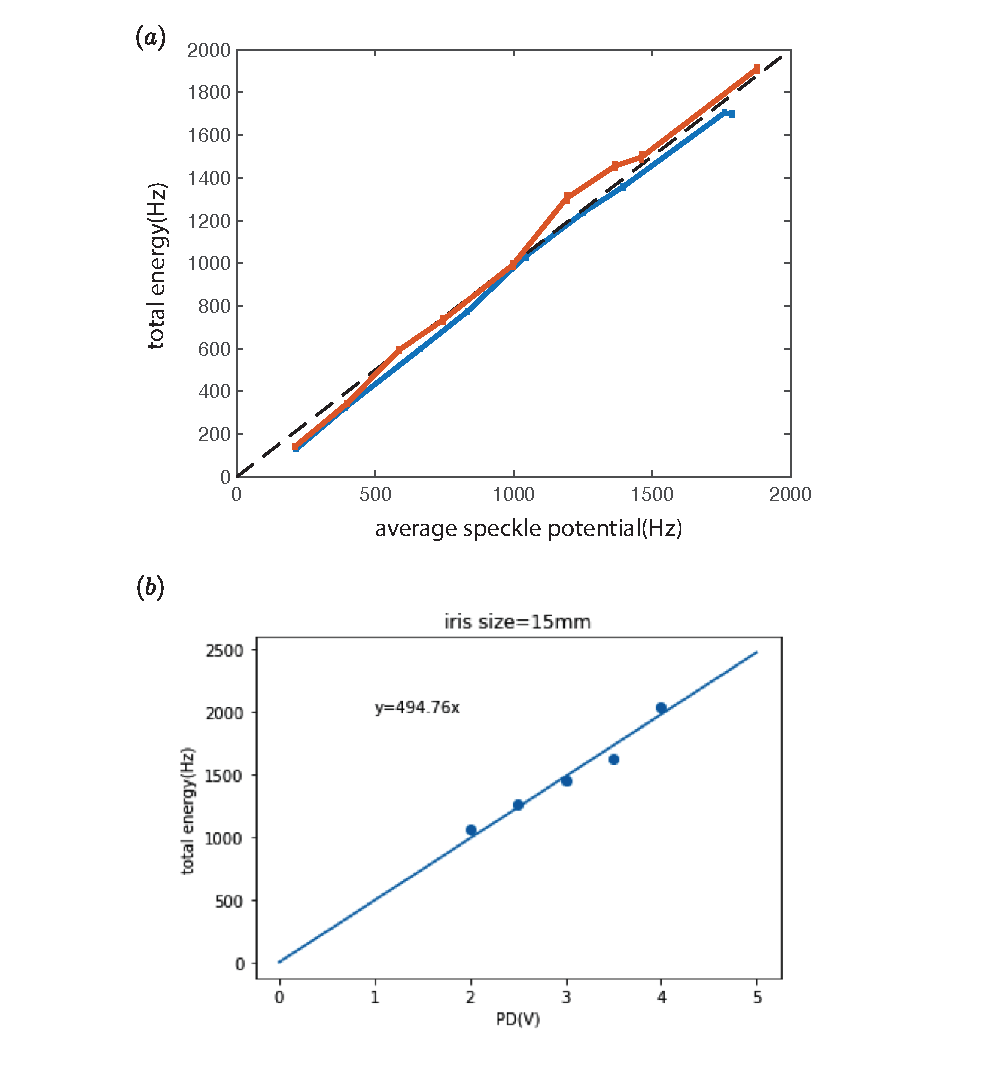
\includegraphics{Chapter6_secs/average_speckle_potential.pdf}
    \caption{Calibration of the average speckle potential depth. (a). In the numerical simulation, the average total energy inferred from the momentum distribution after $20\ {\rm ms}$ free evolution is plotted against the known average speckle potential depth. The red curve and the blue curve are for the speckle potentials with $k_c = 0.80k_r$ and $k_c=1.48k_r$, respectively. The dashed line is diagonal. (b). In the experiment, the average total energy computed from long-term speckle pulsing data is plotted against the PD reading.}
    \label{fig:avg_speckle_poten}
\end{figure*}



